\documentclass{beamer}
%Information to be included in the title page:
\title{Time Complexity}
\author{Neo Wang}
\institute{Westlake High School}
\date{\today}

\AtBeginSection[]
{
  \begin{frame}
    \frametitle{Table of Contents}
    \tableofcontents[currentsection]
  \end{frame}
}

\begin{document}

\frame{\titlepage}

% \begin{frame}
% 	\frametitle{Table of Contents}
% 	\tableofcontents
% \end{frame}

% \section{What is Time Complexity?}

\begin{frame}
\frametitle{Time Complexity}
\subtitle{What is time complexity?}

Time complexity describes the amount of time it takes for a computer to run
an algorithm.

\end{frame}

\begin{frame}
	\frametitle{Time Complexity - Examples}
	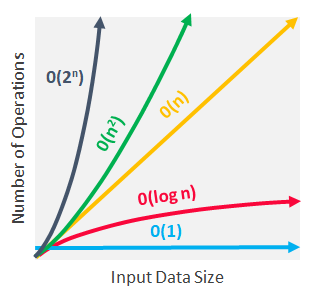
\includegraphics[width=200px]{2021-08-31-13-46-02.png}
	\begin{itemize}
		\item Notice how the number of operations of the algorithm grows as the input size grows.
	\end{itemize}
\end{frame}

\begin{frame}{}
	\frametitle{Common Time Complexities}
	\begin{itemize}
		\item $\mathcal{O}(1)$ - Constant Time. Example: swap two numbers in an array, arithmetic.
		\item $\mathcal{O}(N)$ - Linear Time. Example: looping through
		numbers $[0, \ldots ,n]$
		\item $\mathcal{O}(N^2)$ - Quadratic Time. Example: looping through an
		$N \times N$ matrix.
		\item $\mathcal{O}(\log N)$ - Logarithmic Time. Example: binary search.
		\item $\mathcal{O}(N\log N)$ - Logarithmic Time. Example: merge sort.
		\item Bonus: $\mathcal{O}(\alpha (N))$
	\end{itemize}
\end{frame}

\begin{frame}
	\frametitle{Notes on Time Complexity}
	\begin{itemize}
		\item Time complexity ignores lower forms of computation, because we are
		only trying to describe how the computation scales with input size.
		\item Example: $\mathcal{O}(2N)$ is the same as $\mathcal{O}(N)$, because we ignore the constant
		factor of $2$.
		\item Example 2
		$$\mathcal{O}(N^2\log N + N\log N) = \mathcal{O}(N^2\log N)$$
	\end{itemize}
\end{frame}

\begin{frame}
	\frametitle{Code Example}
	\begin{center}
		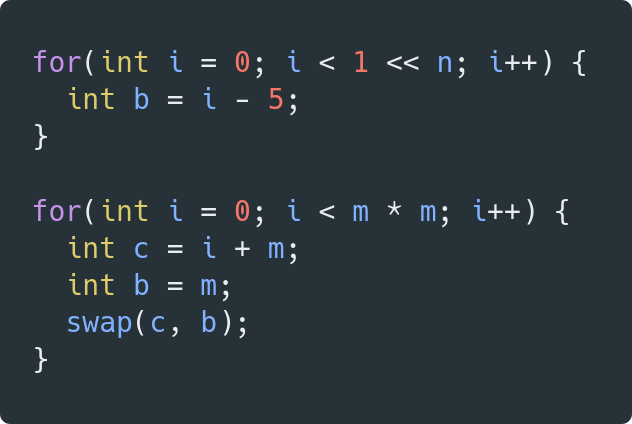
\includegraphics[width=200px]{2021-08-31-14-09-51.png}
	\end{center}
	\begin{itemize}
		\item<1-> Assume $n$ and $m$ are already defined.
		\item<2-> Solution:
		\item<3-> Solution: $\mathcal{O}(2^n + m^2)$
	\end{itemize}
\end{frame}

\begin{frame}
	\frametitle{Why is this useful?}
	Problem: Given an array of $(x, y)$ points, find the closest pair of points.
	There are $N$ points. For reference, looping through each combination of
	points would take $O(N^2)$ time. In around 2 seconds, the computer can process
	in the order of around $5\cdot 10^8$ operations.

	Find out if the time complexity of $\mathcal{O}(N^2)$ would pass for the following:
	
	Problem 1: $N \leq 3000$

	Problem 2: $N \leq 10^5$
\end{frame}

\begin{frame}
	\frametitle{Why is this useful?}

	Problem 1: $N \leq 3000$

	Solution:

	\begin{itemize}
		\item<2-> Solution: Yes, because the time complexity is $O(N^2)$.
		We can estimate our calls by plugging the upper bound of $N(N = 3000)$
		into the equation. $N^2 = 3000^2 = 9\cdot 10^6$ which fits in the bounds
		of $\approx 5\cdot 10^8$ operations.
	\end{itemize}
\end{frame}

\begin{frame}
	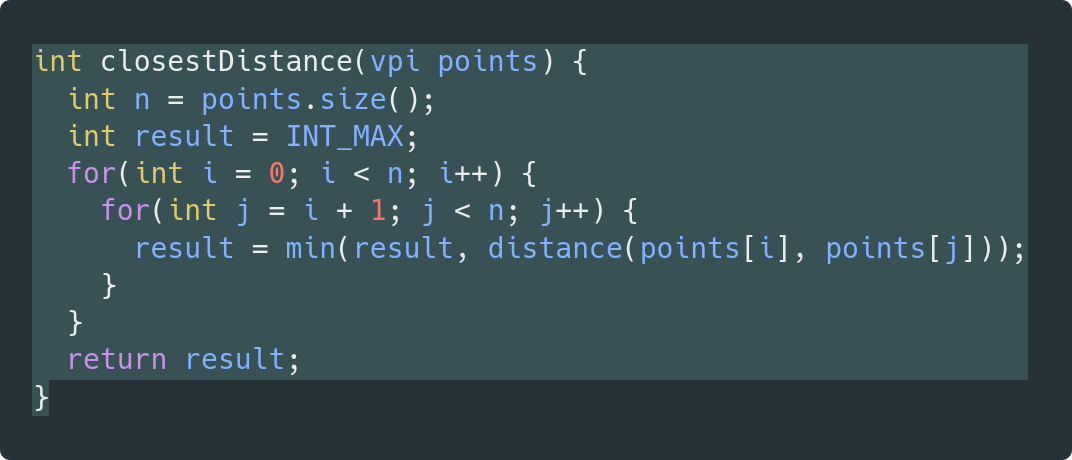
\includegraphics[width=250px]{closestpaireasy.png}
\end{frame}

\begin{frame}
	\frametitle{Why is this useful?}

	Problem 1: $N \leq 10^5$

	Solution:

	\begin{itemize}
		\item<2-> Solution: No, because the time complexity is $O(N^2)$.
		We can estimate our calls by plugging the upper bound of $N(N = 10^5)$
		into the equation. $N^2 = (10^5)^2 = 10^10$ which does not fit in the bound
		of $\approx 5\cdot 10^8$ operations.
	\end{itemize}
\end{frame}

\begin{frame}
	\frametitle{Workaround}
	So what if we want to solve problem 2, since it times out?
	\begin{itemize}
		\item Devise a better algorithm, that passes under $\mathcal{O}(N^2)$
		time complexity.
		\item Costs: Takes a bit of time to implement.
		\item Benefits: Runs faster.
	\end{itemize}
\end{frame}

\begin{frame}
	\frametitle{Workaround}
	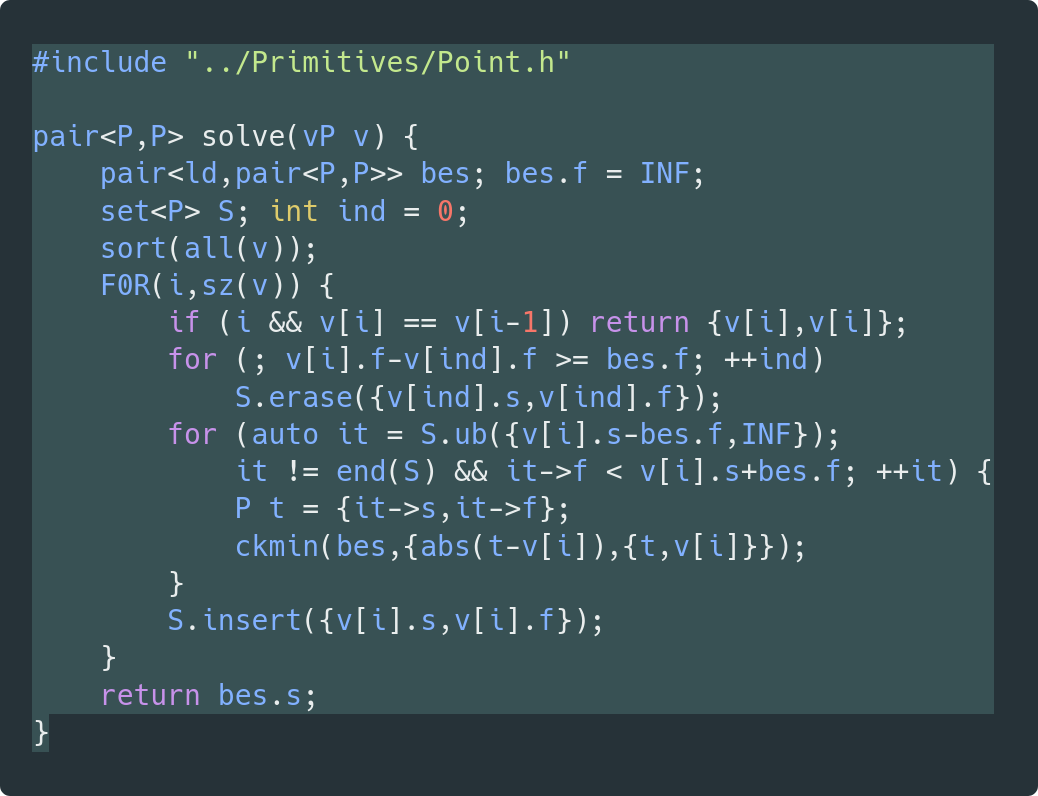
\includegraphics[width=250px]{closestpair.png}
\end{frame}

\begin{frame}
	\frametitle{Advanced Resources}
	\begin{itemize}
		\item \href{https://web.stanford.edu/class/archive/cs/cs106b/cs106b.1172/lectures/11-BigO/11-BigO.pdf}{\color{red}{Stanford CS106B Lecture 11 - Good Introduction}}
		\item \href{https://dl.acm.org/doi/pdf/10.1145/321879.321884}{\color{red}{$\mathcal{O}(\alpha (N))$ proof for Disjoint Set Union w/ Path Compression and Rank}}
		\item \href{https://bit.ly/3tfAf29}{\color{red}{$\mathcal{O}(\log (N))$ proof for Disjoint Set Union w/ Path Compression or Rank}}
	\end{itemize}
\end{frame}
\end{document}